\documentclass[12pt]{article}
\usepackage[utf8]{inputenc}
\usepackage[a4paper, total={6.5in, 8.5in}]{geometry}
% \usepackage{authblk}
% \usepackage{multirow}
\usepackage{graphicx}
% \usepackage{amsmath}
% \usepackage{biblatex}
% \usepackage{rotating}
% \usepackage{ragged2e}
% \usepackage{multicol}
\usepackage{float}
% \usepackage{algpseudocode}
% \usepackage{enumitem}
\usepackage{caption}
\usepackage{subcaption}
\usepackage{hyperref}
\hypersetup{
    colorlinks=true,
    linkcolor=blue,
    }
\usepackage[label=corner]{karnaugh-map}
\usepackage[siunitx, RPvoltages]{circuitikz}
\usetikzlibrary{calc}
\usepackage{tikz, pgfplots}
\usetikzlibrary{positioning}

\title{ALU}
\author{ABRAR JAHIN SARKER}
\date{December 2023}

\begin{document}

\section{\large{Block Diagram}}
\vspace{15mm}
\begin{figure}[H]
    \centering
    \includegraphics[width=0.8\textwidth]{Block_Diagram8.png}
    \caption{ Block Digram of ALU }
    \label{fig:enter-label}
\end{figure}
% \ctikzset{
%     logic ports=ieee,
%     logic ports/scale=1
% }

\section{\large{Complete Circuit Diagram}}

     \begin{figure}[H]
         \centering
         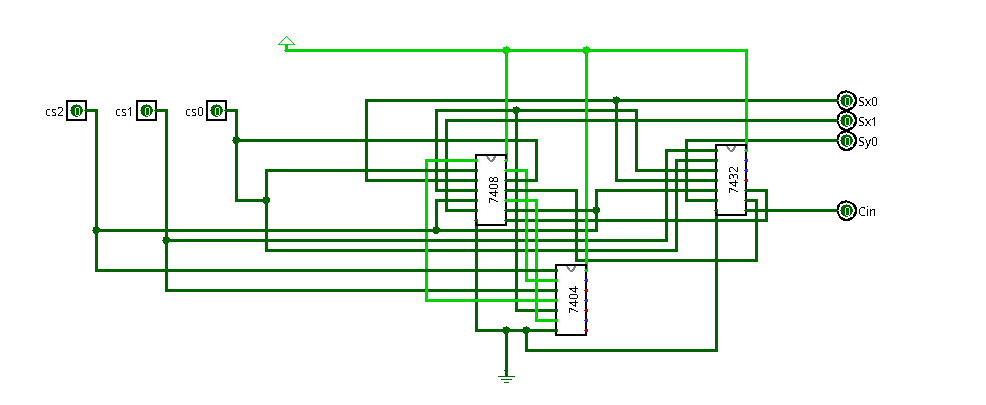
\includegraphics[width=0.8\textwidth]{control_preprocessor.png}
         \caption{Control Processing Unit}
         \label{fig:alu_a}
     \end{figure}
     \begin{figure}[H]
         \centering
         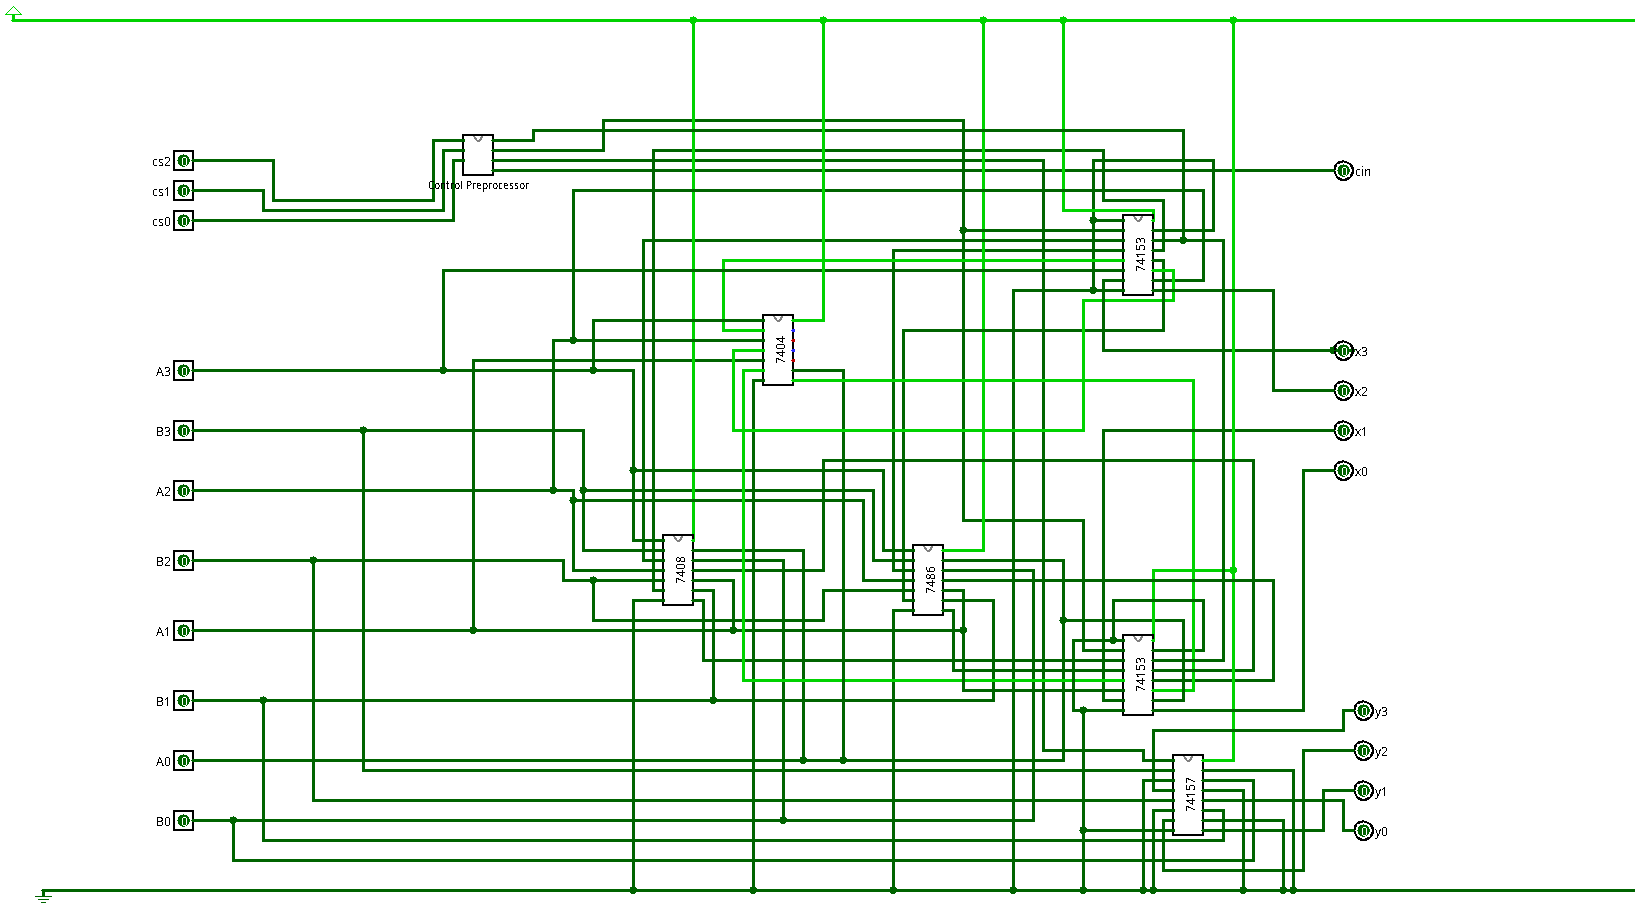
\includegraphics[width=0.8\textwidth]{input_preprocessor.png}
         \caption{Input Processing Unit}
         \label{fig:alu_b}
     \end{figure}
     \begin{figure}[H]
         \centering
         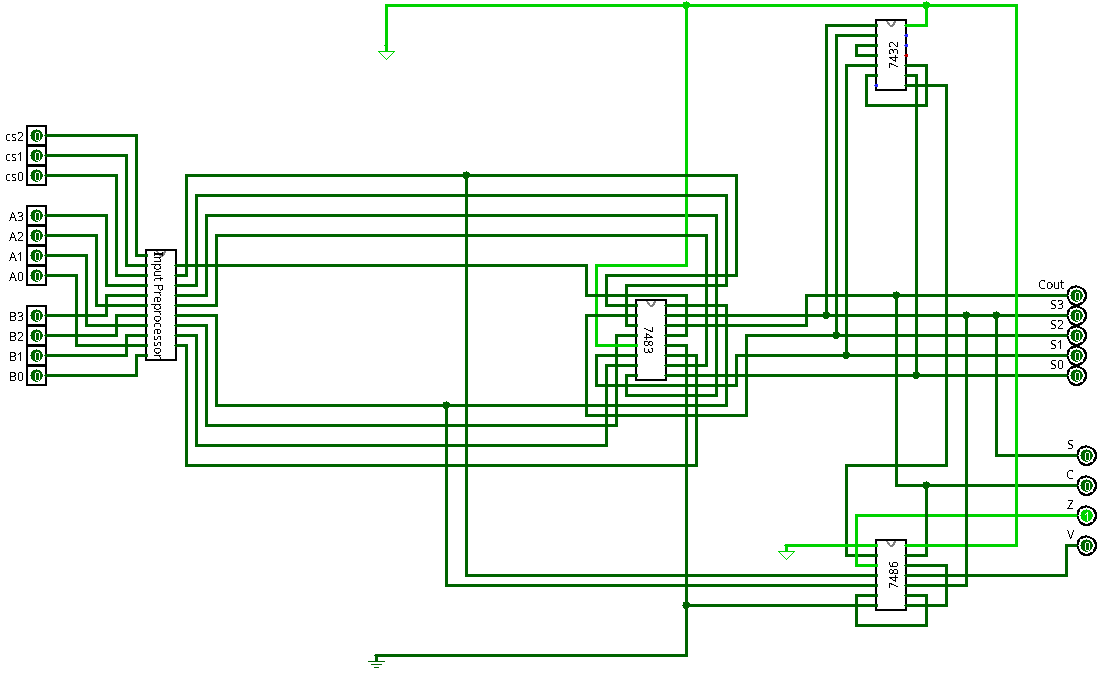
\includegraphics[width=0.8\textwidth]{main.png}
         \caption{The Alu}
         \label{fig:alu_c}
     \end{figure}

\end{document}
